%!TEX root = main.tex
\section{Methods\label{sec:methods}}
\subsection{Background and Motivation}
\par Visual query systems enable users to directly search for visualizations matching certain patterns through an intuitive specification interface. Early work in this space focused on interfaces to search for time series with specific patterns, including TimeSearcher~\cite{Hochheiser2001,Hochheiser2004}, where the query specification mechanism is a rectangular box, filtering out all of the time series that does not pass through it, QuerySketch~\cite{wattenberg2001sketching} and Google Correlate~\cite{mohebbi2011google}, where the query is sketched as a pattern on canvas, filtering out all of the time series that have a different shape. Subsequent work recognized the ambiguity in sketching by studying how humans rank the similarity in patterns~\cite{Eichmann2015,correll2016semantics,Mannino2018} and improving the expressiveness of sketched queries through finer-grained specification interfaces and pattern-matching algorithms~\cite{ryall2005querylines,Holz2009}.
%performed crowdsourced perceptual studies to understand how humans rank similarity in patterns subjectively
% , including the use of soft constraints~\cite{ryall2005querylines} and implicit relaxed selection techniques~\cite{Holz2009}.
% In addition to this ongoing work, recent work have also performed crowdsourced perceptual studies to understand how humans rank similarity in patterns subjectively~\cite{Eichmann2015,correll2016semantics,Mannino2018}.
\par While these systems have been effective in controlled lab studies, they have never been designed and evaluated in-situ on real-world use cases. Even when use cases were involved~\cite{Hochheiser2004,correll2016semantics}, the inclusion of these use cases had a narrow objective and had little influence on the major design decisions of the system. In the context of Munzner's nested model~\cite{munzner2009nested}, this represents the common ``downstream threat'' of jumping prematurely into the deep levels of \textit{encoding, interaction, or algorithm design}, before a proper \textit{domain problem characterization} and \textit{data/operation abstraction design}. In this work, we performed design studies~\cite{lam2012empirical,shneiderman2006strategies,Sedlmair2012} with three different subject areas for \textit{domain problem characterization}. Comparing and contrasting between the diverse set of questions, datasets, and challenges across these three use cases revealed new generalizable insights and enabled us to better understand how VQSs can be extended for novel and unforeseen use cases. Based on these findings, we develop a feature taxonomy for understanding the sensemaking process in VQSs as part of the \textit{data/operation abstraction design}. Finally, we validated the abstraction design with grounded evaluation~\cite{Plaisant2004,Isenberg2008}, where we invite participants to bring in their own datasets and research problems that they have a vested interest in to test our final deployed system. Next, we will describe these two phases of our study in more detail.
%  on our final system ----
% , drawing from ---- grounded evaluation
% validated with usage of deployed system, target users ,
% grounded evaluation
% evaluated on
% participatory design with multiple case studies to ----- target domain, while
% opted for a qualitative mixed-methods approach drawing from ethnographic methods, participatory design, and grounded evaluation~\cite{Plaisant2004,lam2012empirical,shneiderman2006strategies,Sedlmair2012,Isenberg2008} to more thoroughly characterize the problem design space of VQSs and taxonomy abstraction for understanding the sensemaking process in VQSs. Moreover, we performed design studies with three different subject areas with a diverse set of questions, datasets, and challenges to further generalize our findings.
%Most of these systems have not been evaluated in-situ on real-world use cases. Even when design study was performed~\cite{correll2016semantics,Hochheiser2001}, the focus these  narrow use case in mind, and these --- never adopted in practice,either ---did not --- didn't influence the design decisions made to --- . We found there is a genuine need in the community to more thoroughly understand the design space of VQSs and how various components of VQSs are used in practice. In this work, We make use of multiple case studies ....
%\par While these systems have been shown to be effective for visual querying in controlled lab studies, they have not been evaluated in-situ on real-world use cases.
%In this work, we adopted a mixed methods research methodology that draws inspiration from ethnographic methods, iterative and participatory design, and controlled studies~\cite{Plaisant2004,lam2012empirical,shneiderman2006strategies,Muller1993} Participatory design has been successfully used in the development of interactive visualization systems in the past~\cite{Aragon2008,Chuang2012}. Sedlmair et al. \cite{Sedlmair2012} advocate that design study methodology is suitable for use cases in which the data is available for prototyping, but the task is only partially known and the information is partially in the user's head.
%to understand how VQSs can be used in scientific data analysis. %In that regard, our scientific use cases with VQS is well-suited for a design study methodology, as we learn about the scientist's data and analysis requirements and design interactions that helps users translate their ``in-the-head'' specifications into actionable visual queries.
\vspace{-10pt}
\subsection{Phase I: Participatory Design}
\par We recruited participants by reaching out to research groups via email and word of mouth, who have experienced challenges in data exploration. Based on our early conversations with analysts from 12 different potential application areas, we narrowed down to three use cases in astronomy, genetics, and material science for our participatory design study, chosen based on their suitability for VQSs as well as diversity in use cases. Six scientists from three research groups participated in the design of \zvpp. On average, participants had more than 6 years of research experience working in their respective fields. Via interviews and cognitive walkthroughs \change{using participant's original analysis workflow}, we identified the needs and challenges of these use cases. % with researchers from the three different scientific research groups
\par For the participatory design study, we built on an existing VQS, \zv~\cite{Siddiqui2017,Siddiqui2017VLDB}, that allowed users to sketch a pattern or drag-and-drop an existing visualization as a query, with the system returning visualizations that had the closest Euclidean distance from the queried pattern. We chose to build on top of \zv, since it was open-source, extensible, and encompassed a large selection of features compared to existing systems, which focused largely on features for pattern and match specification (as compared in Table~\ref{table:relatedwork}). \change{Past research on participatory design have found that the use of functional prototypes is a common and effective way of engaging with participant and provide a starting point for participatory design~\cite{Ciolfi2016}. Our motivation for providing a functional prototype at the beginning of the participatory design sessions is to showcase capabilities of VQSs. Especially since VQSs are not common in the existing workflows of these scientists, participants may not be able to imagine their use cases without a starting point.}
%The details of the system is described in \cite{Siddiqui2017,Siddiqui2017VLDB}, which focused on the system and scalability aspects of the VQSs.

 %Table~\ref{table:relatedwork} summarizes the list of features offered by these existing systems.
%  that ---
% identified potential opportunities for VQSs
% and potential opportunities for VQSs
% We initially spoke to analysts from 12 different potential application areas and narrowed down to three use cases in astronomy, genetics, and material science for our participatory design study, based on their suitability for VQS as well as diversity in use cases. Six scientists from three research groups participated in the design of \zv. On average, participants had more than 8 years of research experience working in their respective fields. %\techreport{We list the participants in Table~\ref{participants}, and will refer to them by their anonymized ID as listed in the table throughout the paper.}
% \par Given our early conversations with participants, we built a basic VQS to serve as the functional prototype in the design study. This early VQS prototype allowed users to sketch a pattern or drag-and-drop an existing visualization as a query, then the system would return visualizations that had the closest Euclidean distance from the queried pattern. The details of the system is described in \cite{Siddiqui2017,Siddiqui2017VLDB}, which focused on the system and scalability aspects of the VQSs.
% 	% \begin{figure}[ht!]
% 	% \centering
% 	% 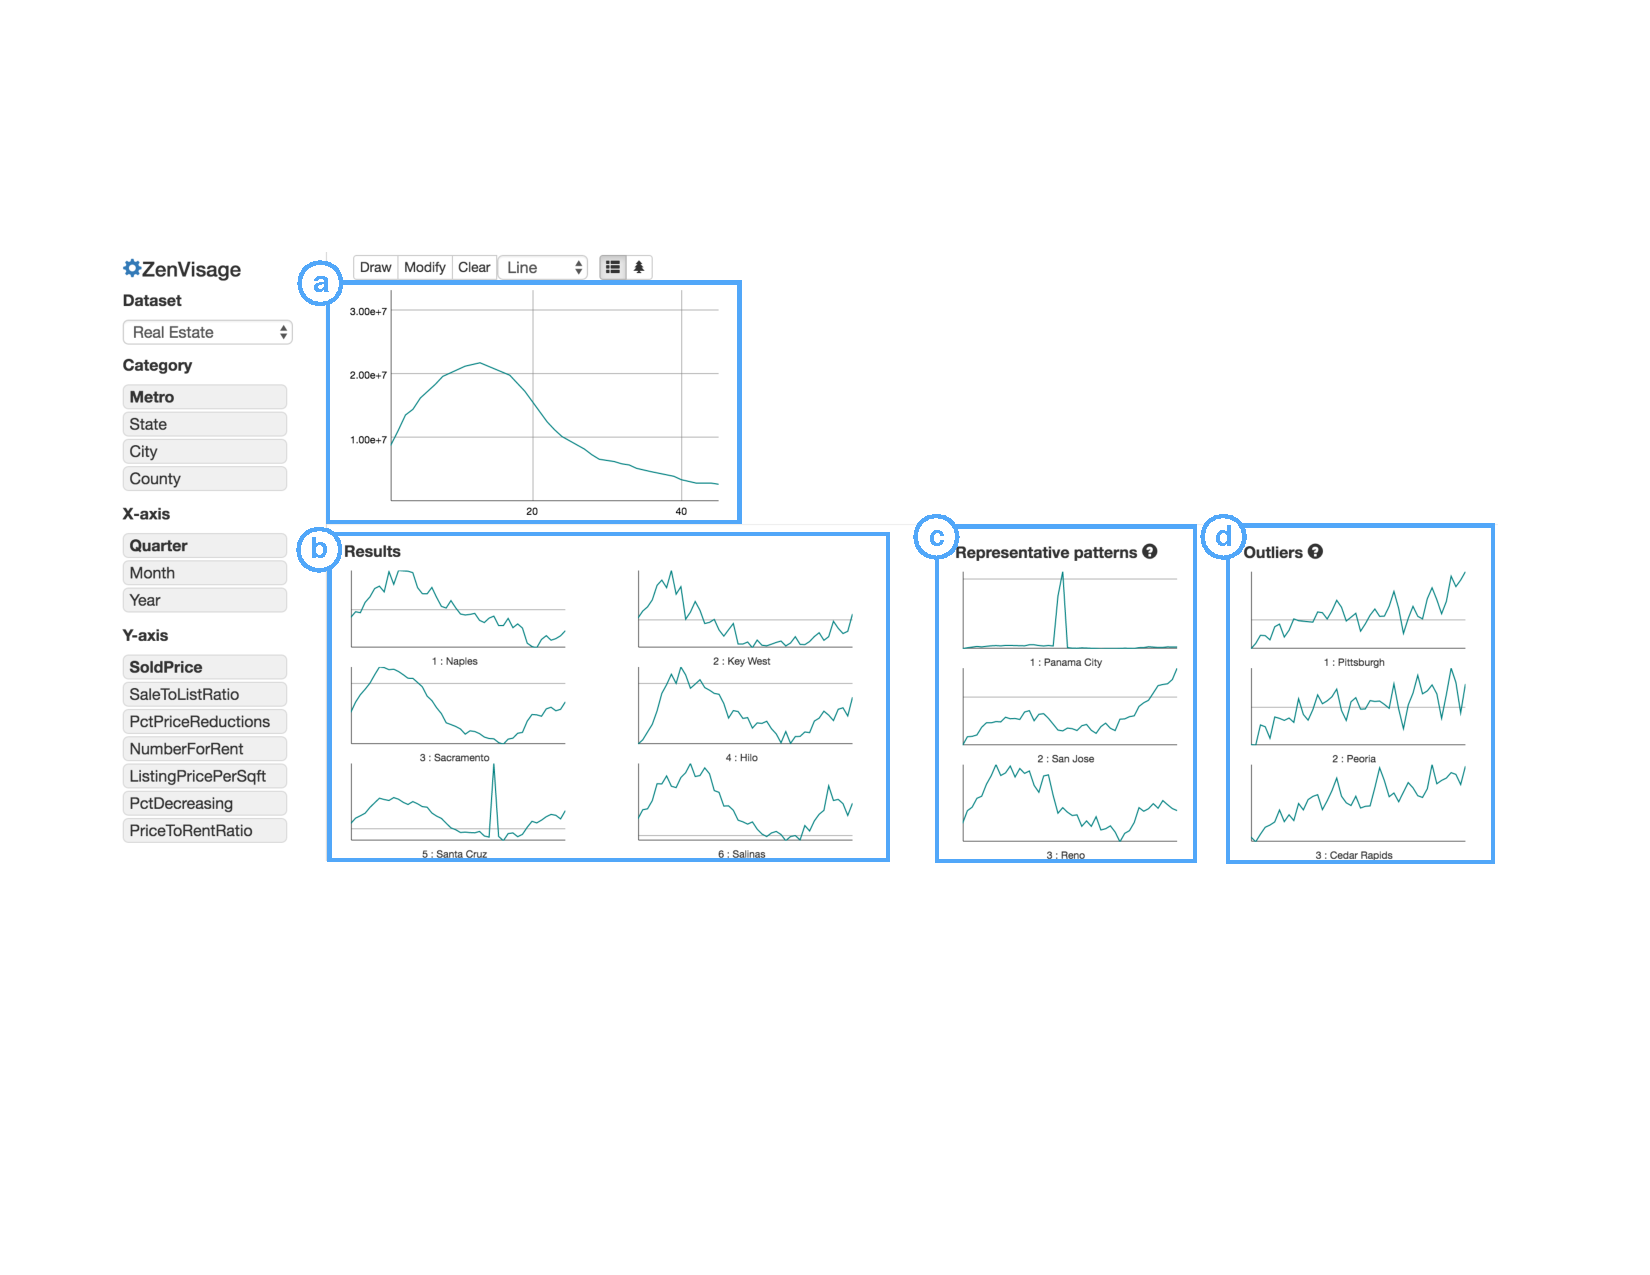
\includegraphics[width=\linewidth]{figures/oldZV_nozql.pdf}
% 	% \caption{The \zv prototype allowed users to sketch a pattern in (a), which would then return (b) results that had the closest Euclidean distance from the sketched pattern. The system also displays (c) representative patterns obtained through K-Means clustering and (d) outlier patterns to help the users gain an overview of the dataset.}
% 	% \label{oldZV}
% 	% \end{figure}
% \par The use of functional prototypes is common and effective in participatory design to provide a starting point for the participants, as studied by Ciolfi et al.\cite{Ciolfi2016}. %For example, Ciolfi et al.\cite{Ciolfi2016} studied two different alternatives to co-design (starting with open brief versus functional prototype) in the development of museum guidance systems and found that while both approaches were equally fruitful, functional prototypes can make addressing a specific challenge more immediate and focused.
% Our motivation for providing a functional prototype at the beginning of the participatory design sessions is to showcase capabilities of VQSs. Especially since VQSs are not common in the existing workflows of these scientists, participants may not be able to imagine their use cases without a starting point.
\par During participatory design, we collaborated with each team closely with an average of two meetings per month, where we learned about their datasets, objectives, and \change{what additional VQS features} could help address their research questions. \change{Since essential features that were crucial for effective exploration were lacking in the original \zv and under development in \zvpp, we did not provide a deployed prototype for participants to actively use on their own during the participatory design period. Instead, as we iterated on the design of these features, relevant functionalities from the intermediate versions of \zvpp were demonstrated to the participants to elicit feedback on how these VQS features could better support their scientific goals.} A summary timeline of our collaboration with participants over a year and features inspired by their use cases can be found in Figure \ref{timeline}. %During these sessions, we discussed and iterated on the design of additional features for \zvpp.
%Participants provided datasets they were exploring from their domain, whereby they had a vested interest in using a VQS to address their own research questions.
Through this process, we identified and incorporated more than 20 desired features into the new version of our VQS, \zvpp, described more in Section~\ref{sec:pd_findings}.
\vspace{-10pt}
\begin{table}[h!]
  \centering
  \vspace{-10pt}
  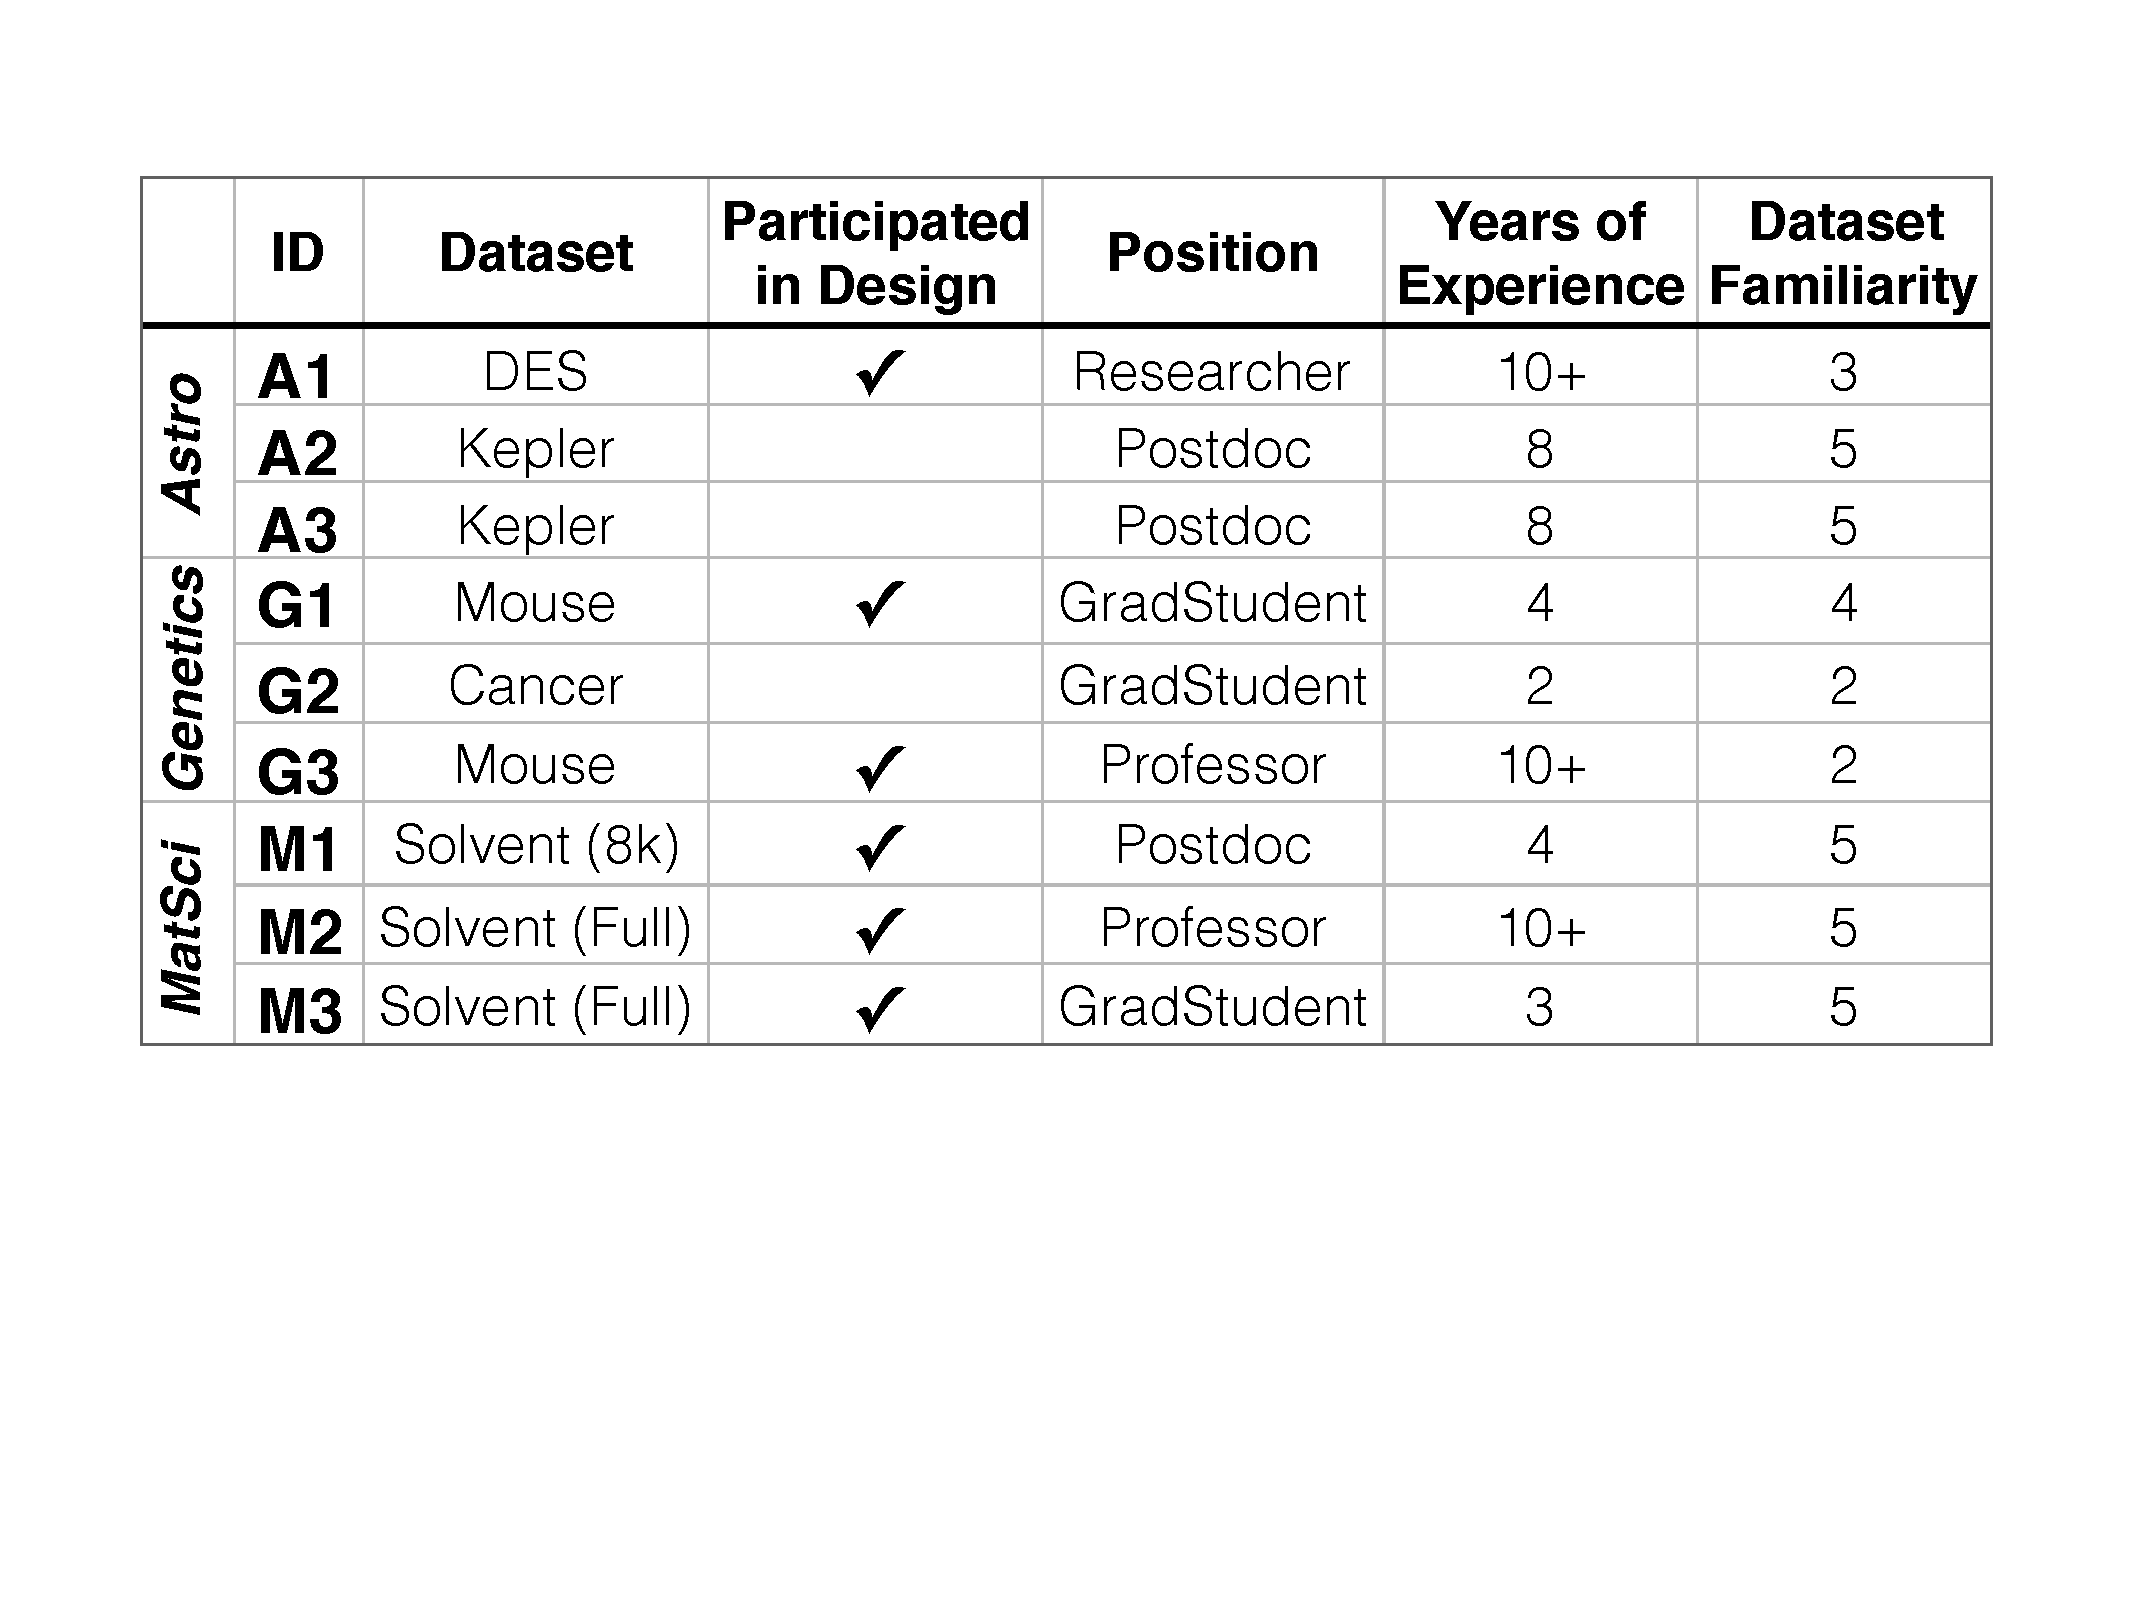
\includegraphics[width=\linewidth]{figures/participant_info.pdf}
  \caption{Participant information. The Likert scale used for dataset familiarity ranges from 1 (not familiar) to 5 (extremely familiar).}
  \label{participants}
  \vspace{-15pt}
\end{table}
\subsection{Phase II: Evaluation Study}
% \par Visualization systems are often evaluated using controlled studies that measure the user's performance against an existing visualization baseline~\cite{Plaisant2004}. Techniques such as artificially inserting ``insights'' or setting predefined tasks for example datasets work well for objective tasks, \techreport{such as debugging data errors~\cite{kandel2011wrangler,Patel2010},} but they are unsuitable for trying to learn about the types of real-world queries users may want to pose on VQSs. %Due to the unrealistic nature of controlled studies, many have proposed using a more multi-faceted, ethnographic approach to understand how analysts perform visual data analysis and reasoning~\cite{Plaisant2004,lam2012empirical,shneiderman2006strategies,munzner2009nested,Sedlmair2012}.
At the end of our participatory design study, we performed a qualitative evaluation to study how analysts interact with different VQS components in practice. In order to make the evaluation more realistic, we invited participants to use datasets that they have a vested interest in exploring to address unanswered research questions. As shown in Table~\ref{participants}, the evaluation study participants included the six scientists from participatory design, along with three additional ``blank-slate'' participants who had never encountered \zvpp before. \change{The use of all or a subset of the project participants (e.g., stakeholders) as evaluation participants is common in participatory design~\cite{Bossen2016}.} \change{Since the participatory design subjects acted as informants and did not actively try out the system on their own,} the evaluation study was the first time that all participants used \zvpp to explore their datasets.
%\ccut{While participatory design subjects actively provided feedback on \zvpp with their data, they only saw us demonstrating their requested features and explaining the system to them, rather than actively using the system on their own. So}
\par Evaluation study participants were recruited from each of the three aforementioned research groups, as well as domain-specific mailing lists. Prior to the study, we asked potential participants to fill out a pre-study survey to determine eligibility. Eligibility criteria included: being an active researcher in the subject area with more than one year of experience, and having worked on a research project involving data of the same nature used in participatory design. \change{None of the participants received monetary compensation, as this is not a common practice for participatory design with stakeholders.} \cite{As detailed in Table~\ref{participants},} the nine participants brought a total of six different datasets to the study. \cut{The research questions and objectives of the participants were diverse even among the same subject area. Examples included understanding gene expression profiles of breast cancer cells after a particular treatment and comparing common patterns among stars that exhibit planetary transits versus stars that do not.\techreport{from the Kepler space telescope\footnote{\url{www.nasa.gov/mission_pages/kepler/main/index.html}}.}}
% Four of the evaluation studies were conducted remotely. Participants had the option of exploring their own dataset or an existing dataset that they provided to us during the participatory design process. All three blank-slate participants opted to explore their own datasets.
 %After loading their dataset, we emailed them a screenshot of a visualization from our tool to verify that we configured the system to meet their needs.
\par At the start, participants were provided with an interactive walk-through explaining the system details and given approximately ten minutes for a guided exploration of \zvpp with a preloaded real-estate example dataset from Zillow \cite{zillow}.\techreport{This dataset contained housing data for various cities, metropolitan areas, and states in the U.S. from 2004-15.} After familiarizing themselves with the tool, we loaded the participant's dataset and encouraged them to talk-aloud during data exploration and use external tools. If the participant was out of ideas\ccut{ for three minutes}, we suggested one of the ten main VQS functionalities \techreport{\footnote{query by sketching, drag-and-drop, pattern loading, input equations, representative and outliers, narrow/ignore x-range options, filtering, data smoothing, creating dynamic classes,  data export}}that they had not yet used. If any of these operations were not applicable to their specific dataset, they were allowed to skip the operation after having considered how it may or may not be applicable to their workflow. The user study ended after they covered all ten main functionalities. On average, data exploration lasted for 63 minutes. After the study, we asked them open-ended questions about their experience.% and suggested an appropriate choice of axis to begin the exploration.
%\par During the exploration phase, participants were informed that they could use other tools as needed.
